% ============================================================
% S2 导学件量产·批4 件2 —— 1.2.3 直线与平面的夹角（课时8 导学件）
% 轮4 成卷·S2 批4｜2026-09-12｜生成链：xelatex main.tex（两遍）→ python render.py（150dpi → png/pageN.png）
%
% 模板承 v11 样张族（经 课时02 首件／批1／批2／批3）：六宏＝原样拷贝（L1 冻结参数零改动，md5 与 课时06 一致）；
%   课时页形制与局部宏（\pingtou/\liubai/\zhankong）照抄 课时06/课时07。
% 图＝源图位图（禁绘三维，公共规则§5）：figs/ 十件自 讲练件（上）定稿 docx word/media/ 原件解包
%   （sub3_B_11/image57/60/62/63/64/65/66/68/70，元素607/619/637/652/653/663/680/689/690/702，未改绘；
%   与批3解包逐字节 cmp 过），alt 缺失＝就绪报告 §四-5 照登；源 extent 微档（3~9mm）＝源件版式病，
%   成品按像素比例放大至栏内可读宽（批3 §2.5 口径）。
%   组装病自查（批3 §〇三例）：本件不用局部 \fig 宏（图片行恒用定宽 \includegraphics 直式）；
%   选项双盒统一 0.5\linewidth−1em／0.25\linewidth−0.5em，长选项独行（件1 已修一例）；
%   缺字形预检＝「刍/甍」等冷僻字以编译 Missing character 门实测为准，命中则文本化复原并登记。
%
% 取材链登记（盘点结论，详见 成卷/导学件/批4值台账.md）：
%   ① 讲练件（上）§1.2.3 讲部实态（dump_docx --slice 601:726 取证＝工作区/_tmp批4S2量产0912/讲上-1.2.3全文.txt）：
%      知识讲解＝1.2.3-1〔进〕三余弦定理（含证明与推论·最小角定理）＋1.2.3.2 方法讲解（大招2）；
%      题型例题 7 段 8 题（1.2.3.2.1-1～1.2.3.2.7-8，简1＋中6＋难1）。节净 8 题全部入本件课中探究
%      （例1×5＋变式1×3 同文位）。
%   ② 探究点随讲部题型段归并＝5 个：一 求线面角的值·三余弦定理（.2.2 段 -3 例〔简单〕／.2.1 段 -2 变〔中档〕）；
%      二 向量法线面角与参数存在性（.2.1 段 -1 例·三选开放／变式命制）；三 折叠问题中的线面角
%      （.2.3 段 -4 例／.2.6 段 -7 变·刍甍双问，折叠同族归并）；四 线面角与范围最值（.2.4 段 -5 例／
%      .2.5 段 -6 变·折叠端值，最值/范围同族归并）；五 线面角综合最值（.2.7 段 -8 例〔难〕／变式命制）。
%      大招2 方法讲解（元素610–615）不独立成点，其定理本体与图入 ZSD三（同文化用）。
%   ③ 与课时08 练习轴 16 题互斥口径：讲部 8 题中 -1/-2/-3/-7/-8 五题与练习轴第 7/4/5/8/10 题同文
%      （题源＝讲部同号，A-2「照用」同题双印登记，题数不并计）；-4/-5/-6 未入练习轴（16 题题源逐查无）。
%      命制位＝判断 5＋变式两处（探究二/五）＋评价 5＝12 题，与 16 题逐题零同文（题面/设问形态均异，断言见台账）。
%   ④ 课前预习 ZSD一/二＝教材 1.2.3 正文同文化用（_tmp教材全文.txt 页44–47 实证：垂直所成角 90°、平行或在面内
%      0°、斜线与射影所成角＝线面角、最小角定理、A′B′=ABcosθ、θ=π/2−⟨v,n⟩ 或 ⟨v,n⟩−π/2、
%      sinθ=|cos⟨v,n⟩|——白名单·教材原文）；ZSD三＝讲部 1.2.3-1 三余弦定理同文化用（含证明链图）；
%      判断/评价＝恒命制位，逐题亲算登台账。
%   ⑤ 句末标点：同文段承源「.」，新命制句用「．」（G8 成卷轮统一清扫，本件不单点改）。
% 编译门：三 0（error＝0／Overfull＝0／Missing character＝0，Underfull 仅计数）——读数见批4值台账。
% ============================================================
\documentclass[fontset=none]{ctexart}
\usepackage{qp-m3} % 换装：六宏→qp-m3 单包（钉后版 md5 7c3930362be8a0a2bdf21bbf8ac16573，两补钉随版）

% ================= 页脚参数宏（qp-headfoot 文件头明示的复用入口，非模块语义改动） =================
\renewcommand{\qpzhangming}{第一章\quad 空间向量与立体几何}
\renewcommand{\qpjianming}{导学件}
\renewcommand{\qpceming}{高中数学\quad 选择性必修第一册(人教B版)} % 换装回钉：qp-m3 默认册名＝选必二，防页脚漂移（试迁规约）

% ================= 局部宏（照抄 v11 导学增量/main.tex 冻结定义；不动公共模块） =================
% 课堂评价组头（XB-02 \zhenhead 同构：\biaoqian 1.3× 标签＋仿宋说明行；恒 5 题说明）
% 局部宏 \pingtou 已由 qp-m3 收编（等值定义），依换装方案§1.4 预删防撞名
% 书写留白＋斜置浅灰水印（导学案正文属性：答案另册→正文留书写位；斜置 25°／black!12）
% 长度 \liubaoh 已由 qp-m3 分配，预删防重复定义
% 局部宏 \liubai 已由 qp-m3 收编（等值定义），依换装方案§1.4 预删防撞名
% 纯书写占位留白（无水印）
% 局部宏 \zhankong 已由 qp-m3 收编（等值定义），依换装方案§1.4 预删防撞名

% 纯题版孤行抑制（正装三裁①）：小结②操作/③收束独立段，pure 档整段隐藏，含详解版不受影响
\newcommand{\bindpx}[1]{\ifshowans\bindp{#1}\fi}

\begin{document}

% ============================================================
% 课时页（第8课时；五段闭环，承 v11 导学增量课时页样板形制）
% ============================================================
\keshi{第8课时\quad 直线与平面的夹角}
\mubiaoline
\mubiaomu{1}{理解直线与平面所成的角的定义(含垂直\(90^{\circ}\)、平行或在该平面内\(0^{\circ}\)的规定)，掌握最小角定理与射影长公式；}
\mubiaomu{2}{掌握用直线的方向向量与平面的法向量求直线与平面所成的角的方法\(\sin\theta=|\cos\langle\overrightarrow{v},\overrightarrow{n}\rangle|\)，会处理已知线面角求参数的问题；}
\mubiaomu{3}{了解三余弦定理，会用三余弦定理与向量法解决折叠、取值范围与最值等线面角综合问题，体会化归与转化的思想.}

\vspace{1.7mm}
\begin{multicols}{2}
\emergencystretch=1em

% ---------- 课前预习（知识导学填空＋诊断分析挂每个知识点之后；ZSD一/二＝教材 1.2.3 正文同文化用，ZSD三＝讲部 1.2.3-1 三余弦定理同文化用） ----------
\huaxing{课}{前}{预}{习}{知识导学\quad 素养初识}

\zsd{一}{直线与平面所成的角}

\tiaomu{1}{位置的规定：如果一条直线与一个平面垂直，则称这条直线与这个平面所成的角为\kongbai{}；如果一条直线与一个平面平行，或直线在平面内，则称这条直线与这个平面所成的角为\kongbai{}．}

\tiaomu{2}{斜线与平面所成的角：如图，如果直线\(AB\)是平面\(\alpha\)的一条斜线，\(B\)为斜足，\(A'B\)是直线\(AB\)在平面\(\alpha\)内的射影，则\kongbai{}就是直线\(AB\)与平面\(\alpha\)所成的角．直线与平面所成的角也称为它们的夹角．因此，直线与平面所成角\(\theta\)的范围是\kongbai{}．}

\tiaomu{3}{最小角定理与射影长：平面的斜线与平面所成的角，是斜线和这个平面内\kongbai{}所成角中最小的角；当线段\(AB\)所在的直线与平面\(\alpha\)所成的角为\(\theta\)，且\(AB\)在平面\(\alpha\)内的射影为\(A'B'\)时，有\(A'B'=\)\kongbai{}．\zhuzhu{经过平面外同一点所作的平面的多条斜线中，斜线段长、射影长及斜线与平面所成的角，只要有一个相等，则另外两个也对应相等.}}

\zhenhead{判断正误(正确的打\gou{},错误的打\cha{})}

\zhentib{(1)}{若两条直线都平行于同一个平面，则这两条直线平行．}

\begin{ansblock}[导-课时08-判1]
% ans:导-课时08-判1
\ansitem{(1)}{$\times$}
\end{ansblock}

\zhentib{(2)}{任意一条线段在一个平面内的射影仍是线段．}

\begin{ansblock}[导-课时08-判2]
% ans:导-课时08-判2
\ansitem{(2)}{$\times$}
\end{ansblock}

\zsd{二}{用空间向量求直线与平面所成的角}

\tiaomu{1}{向量公式：设\(\overrightarrow{v}\)是直线\(l\)的一个方向向量，\(\overrightarrow{n}\)是平面\(\alpha\)的一个法向量，直线\(l\)与平面\(\alpha\)所成角的大小为\(\theta\)，则\(\theta=\frac{\pi}{2}-\langle\overrightarrow{v},\overrightarrow{n}\rangle\)或\(\theta=\langle\overrightarrow{v},\overrightarrow{n}\rangle-\frac{\pi}{2}\)；特别地，\(\cos\theta=\)\kongbai{}，\(\sin\theta=\)\kongbai{}．\zhuzhu{线面角等于方向向量与法向量夹角的余角(或其补角的余角)；忘取绝对值是求线面角的最常见错误.}}

\zhenhead{判断正误(正确的打\gou{},错误的打\cha{})}

\zhentib{(1)}{若直线\(l\)的方向向量与平面\(\alpha\)的法向量的夹角为\(60^{\circ}\)，则\(l\)与\(\alpha\)所成的角为\(60^{\circ}\)．}

\begin{ansblock}[导-课时08-判3]
% ans:导-课时08-判3
\ansitem{(1)}{$\times$}
\end{ansblock}

\zhentib{(2)}{设\(\overrightarrow{v}\)是直线\(l\)的方向向量，\(\overrightarrow{n}\)是平面\(\alpha\)的法向量，\(l\)与\(\alpha\)所成角为\(\theta\)，则\(\sin\theta=|\cos\langle\overrightarrow{v},\overrightarrow{n}\rangle|\)．}

\begin{ansblock}[导-课时08-判4]
% ans:导-课时08-判4
\ansitem{(2)}{\(\surd\)}
\end{ansblock}

\zsd{三}{三余弦定理}

\tiaomu{1}{三余弦定理：如图，\(O\)为平面\(\alpha\)内一点，直线\(l\)是平面\(\alpha\)的一条过点\(O\)的斜线，\(OB\)为\(OA\)在平面\(\alpha\)内的投影，\(OC\)为平面\(\alpha\)内任一直线，则\(\cos\angle AOC=\)\kongbai{}．}

\bindp \par\vspace{1.9mm}\penalty10000\noindent\makebox[\linewidth][c]{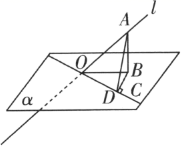
\includegraphics[width=34.0mm]{figs/sub3_B_11.png}}\par\vspace{-1.0mm}\penalty10000

\tiaomu{2}{应用要点：三余弦定理构建了「水平面」上的\(\angle COB\)、「竖直面」上的\(\angle AOB\)以及「斜面」上的\(\angle AOC\)的余弦之间的关系，知道其中两个角就能求出另外一个角，可用于求直线与平面所成的角等问题；特点：连续两次投影．}

\begin{ansblock}[导-课时08-预习填空]
% ans:导-课时08-预习填空
\ansnote{预习填空}{知识点一：\(90^{\circ}\)；\(0^{\circ}\)；\(\angle ABA^{\prime}\)；\([0^{\circ},90^{\circ}]\)；所有直线；\(AB\cos\theta\)。知识点二：\(\sin\langle\overrightarrow{v},\overrightarrow{n}\rangle\)；\(\left|\cos\langle\overrightarrow{v},\overrightarrow{n}\rangle\right|\)。知识点三：\(\cos\angle AOB\cdot\cos\angle BOC\)。}
\end{ansblock}

\zhenhead{判断正误(正确的打\gou{},错误的打\cha{})}

\zhentib{(1)}{平面的斜线与平面所成的角，是这条斜线与该平面内所有直线所成角中最小的角．}

\begin{ansblock}[导-课时08-判5]
% ans:导-课时08-判5
\ansitem{(1)}{\(\surd\)}
\end{ansblock}

\liubai[4mm]{此处书写}

% ---------- 课中探究（探究点5个＝讲部7段归并5个；例1/变式1同文位＝讲部题面逐字(记号LaTeX化)；素养小结＝讲部题型通式编注化用） ----------
\huaxing{课}{中}{探}{究}{考点探究\quad 素养小结}

\tjdnr{一}{求线面角的值(三余弦定理)}{例\textbf{1}}{简单(知识点三)}{正四面体\(ABCD\)中，\(O\)为\(\triangle BCD\)的重心，则\(\cos\angle ABO=\)\kongbai{}.}

\begin{ansblock}[导-课时08-探1-例1]
% ans:导-课时08-探1-例1
\ansnote{例1}{\(\dfrac{\sqrt{3}}{3}\)}
\end{ansblock}

\liB{变式\textbf{1}}{中档(知识点三)}{}{如下图所示，在平行六面体\(ABCD-A_{1}B_{1}C_{1}D_{1}\)中，底面\(ABCD\)为矩形，侧棱\(AA_{1}\)与\(AD\)、\(AB\)均成\(60^{\circ}\)角，则侧棱\(AA_{1}\)与底面\(ABCD\)所成的角为\kongbai{}．}

\bindp \par\vspace{1.9mm}\penalty10000\noindent\makebox[\linewidth][c]{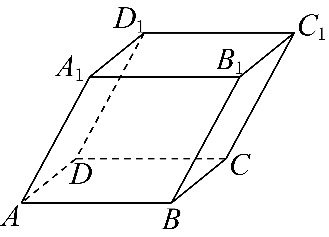
\includegraphics[width=36.0mm]{figs/image60.png}}\par\vspace{-1.0mm}\penalty10000

\begin{ansblock}[导-课时08-探1-变式1]
% ans:导-课时08-探1-变式1
\ansnote{变式1}{\(45^{\circ}\)}
\end{ansblock}

\xiaojie{①识别：题干所求角可分解为「斜线与平面所成角＋射影与平面内直线所成角」两级时，判归本题型.}

\bindpx {\kaishu ②操作：确认斜线、斜线在平面内的射影与平面内直线三者的位置，代入三余弦公式\(\cos\angle AOC=\cos\angle AOB\cdot\cos\angle BOC\)(其中\(\angle AOB\)为线面角，\(\angle BOC\)为射影角).}

\bindpx {\kaishu ③收束：由已知两角求第三角；斜线与平面所成的角是全部所成角中最小的.}

\tjdnr{二}{线面角与参数存在性(向量法)}{例\textbf{1}}{中档(知识点二)}{在①\(\angle PAB=60^{\circ}\)；②\(PA\perp PB\)；③\(\angle PAB=120^{\circ}\)这三个条件中任选一个，补充在下面问题中，若问题中的\(\lambda\)存在，求出\(\lambda\)的值；若\(\lambda\)不存在，请说明理由．已知等腰三角形\(PAB\)和正方形\(ABCD\)，\kongbai{}，\(AB=1\)，平面\(PAB\perp\)平面\(ABCD\)，是否存在点\(E\)，满足\(\overrightarrow{PE}=\lambda\overrightarrow{PC}\)，使直线\(DE\)与平面\(PBC\)所成角为\(60^{\circ}\)？}

\bindp \par\vspace{1.9mm}\penalty10000\noindent\makebox[\linewidth][c]{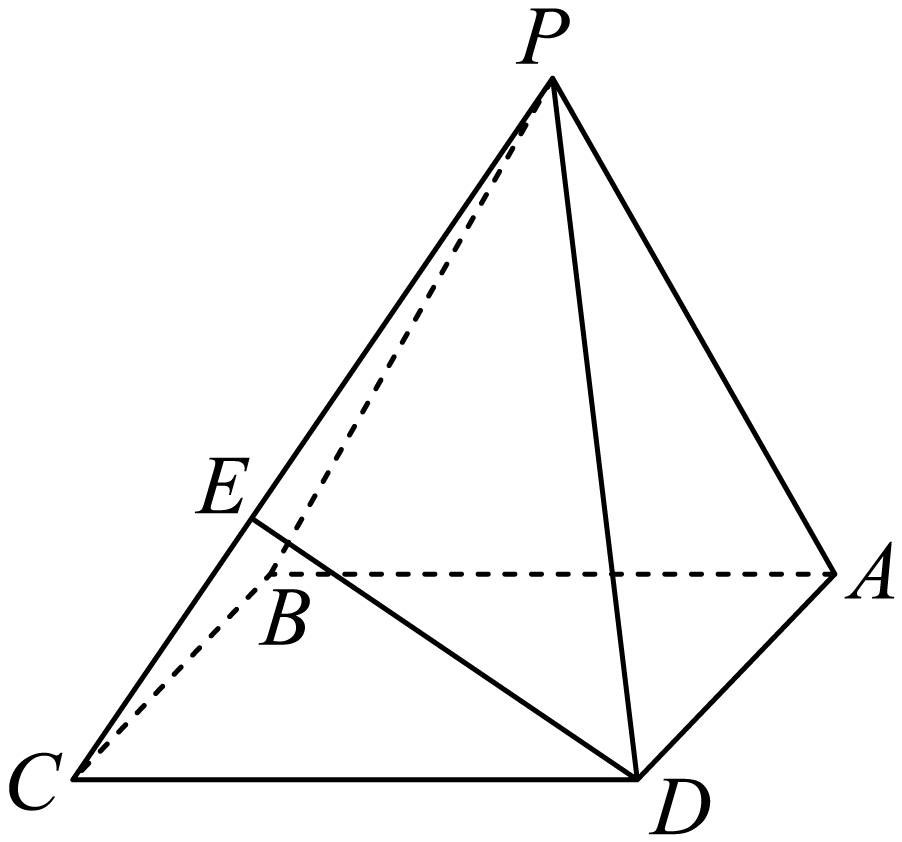
\includegraphics[width=34.0mm]{figs/image57.png}}\par\vspace{-1.0mm}\penalty10000

\liubai[12mm]{解答书写区}

\begin{ansblock}[导-课时08-探2-例1]
% ans:导-课时08-探2-例1
\ansnote{例1}{①\(\lambda=\dfrac{1}{2}\) 或 \(1\)；②③不存在}
\end{ansblock}

\liB{变式\textbf{1}}{简单(知识点二)}{}{若直线\(l\)的方向向量\(\overrightarrow{u}\)与平面\(\alpha\)的法向量\(\overrightarrow{n}\)的夹角为\(120^{\circ}\)，则直线\(l\)与平面\(\alpha\)所成的角为(\kongwei)}

\bindopt {\fontsize{10.5pt}{19pt}\selectfont \makebox[\dimexpr0.25\linewidth-0.5em\relax][l]{A．\(30^{\circ}\)；}\makebox[\dimexpr0.25\linewidth-0.5em\relax][l]{B．\(45^{\circ}\)；}\makebox[\dimexpr0.25\linewidth-0.5em\relax][l]{C．\(60^{\circ}\)；}\makebox[\dimexpr0.25\linewidth-0.5em\relax][l]{D．\(90^{\circ}\)}\par}

\begin{ansblock}[导-课时08-探2-变式1]
% ans:导-课时08-探2-变式1
\ansnote{变式1}{A（\(30^{\circ}\)）}
\end{ansblock}

\xiaojie{①识别：题干求直线与平面所成的角、或以线面角为条件求参数(判断存在性)时，判归本题型.}

\bindpx {\kaishu ②操作：建系写出直线的方向向量并求平面的法向量，由\(\sin\theta=|\cos\langle\overrightarrow{u},\overrightarrow{n}\rangle|\)列式.}

\bindpx {\kaishu ③收束：解出角度或参数；存在性问题按方程是否有解、参数是否落在范围内下结论.}

\tjdnr{三}{折叠问题中的线面角}{例\textbf{1}}{中档(知识点一)}{如下图所示，矩形\(ABCD\)中，\(AB=2\sqrt{2}\)，\(AD=2\)，沿\(BD\)将\(\triangle BCD\)折起，使得点\(C\)在平面\(ABD\)上的射影落在\(AB\)上，则直线\(BC\)与平面\(ABD\)所成的角为\kongbai{}．}

\bindp \par\vspace{1.9mm}\penalty10000\noindent\makebox[\linewidth][c]{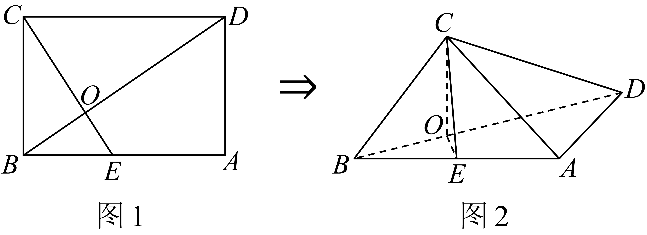
\includegraphics[width=40.0mm]{figs/image62.png}\hspace{2.5mm}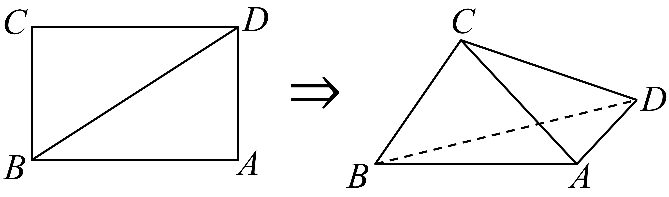
\includegraphics[width=40.0mm]{figs/image63.png}}\par\vspace{-1.0mm}\penalty10000

\begin{ansblock}[导-课时08-探3-例1]
% ans:导-课时08-探3-例1
\ansnote{例1}{\(45^{\circ}\)}
\end{ansblock}

\liB{变式\textbf{1}}{中档(知识点二)}{}{如图1，\(E\)、\(F\)、\(G\)分别是正方形的三边\(AB\)、\(CD\)、\(AD\)的中点，先沿着虚线段\(FG\)将等腰直角三角形\(FDG\)裁掉，再将剩下的五边形\(ABCFG\)沿着线段\(EF\)折起，连接\(AB\)、\(CG\)就得到了一个「刍甍」(如图2)．(1)若\(O\)是四边形\(EBCF\)对角线的交点，求证：\(AO\parallel\)平面\(GCF\)；(2)若二面角\(A-EF-B\)的大小为\(\frac{2}{3}\pi\)，求直线\(AB\)与平面\(GCF\)所成角的正弦值．}

\bindp \par\vspace{1.9mm}\penalty10000\noindent\makebox[\linewidth][c]{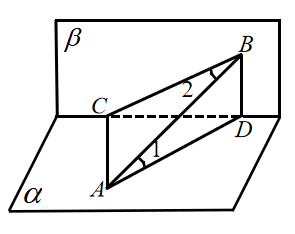
\includegraphics[width=26.0mm]{figs/image66.png}\hspace{2.5mm}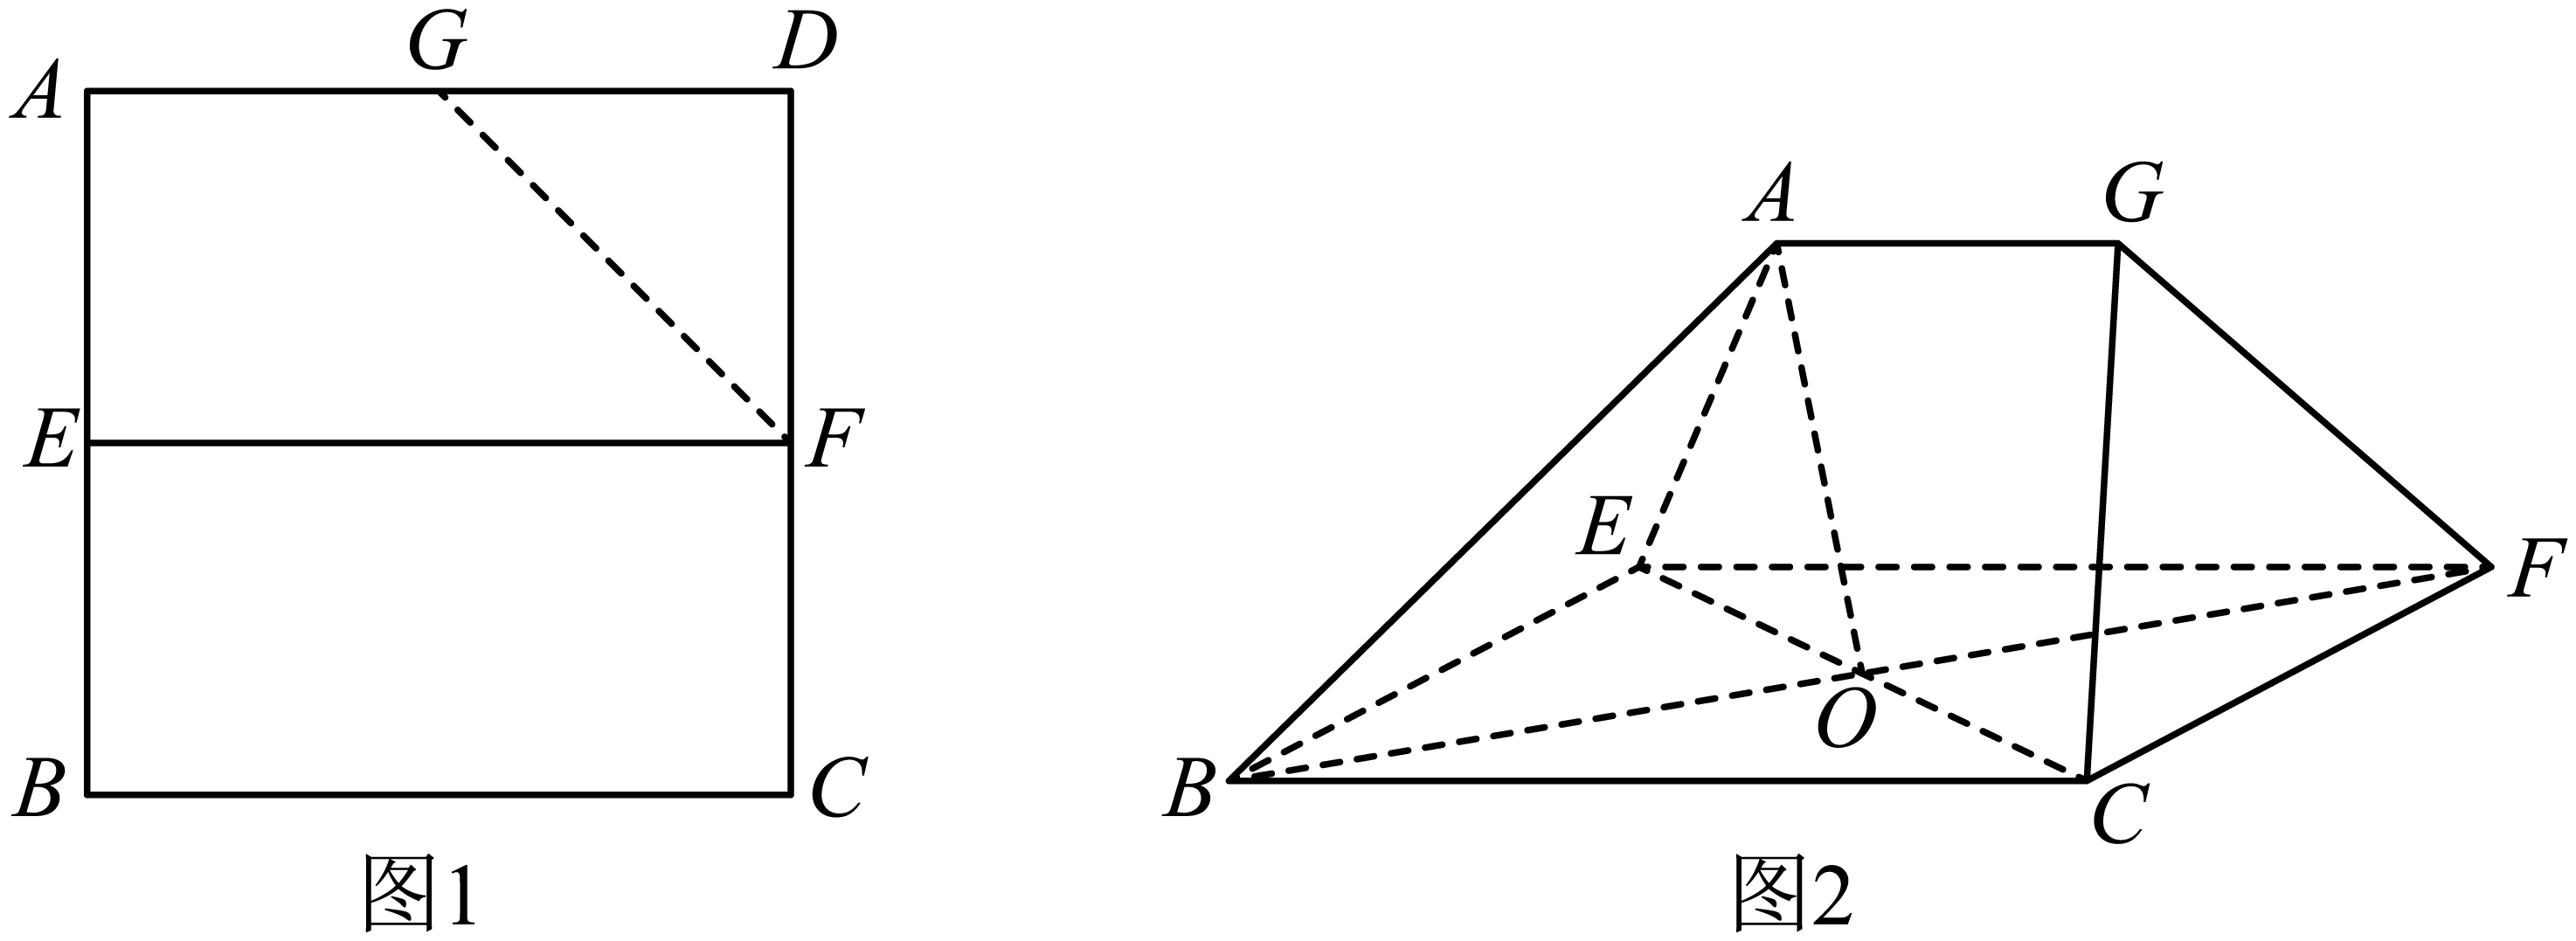
\includegraphics[width=52.0mm]{figs/image68.png}}\par\vspace{-1.0mm}\penalty10000

\liubai[10mm]{解答书写区}

\begin{ansblock}[导-课时08-探3-变式1]
% ans:导-课时08-探3-变式1
\ansnote{变式1}{(1)证明见解析；(2)\(\dfrac{\sqrt{7}}{7}\)}
\end{ansblock}

\xiaojie{①识别：题干把平面图形折成空间体(刍甍等)、要求证明或求折叠后的线面角(线面平行)时，判归本题型.}

\bindpx {\kaishu ②操作：利用折叠前后的不变量与中点、中位线构造平行关系；再由射影位置或二面角条件确定折叠程度，作出垂线(或建系求法向量).}

\bindpx {\kaishu ③收束：线面角即斜线与其射影的夹角，或用\(\sin\theta=|\cos\langle\overrightarrow{u},\overrightarrow{n}\rangle|\)计算，也可用三余弦公式.}

\tjdnr{四}{线面角与范围、最值(三余弦定理)}{例\textbf{1}}{中档(知识点二)}{平行六面体\(ABCD-A_{1}B_{1}C_{1}D_{1}\)中，已知底面四边形\(ABCD\)为正方形，\(\angle A_{1}AB=\angle A_{1}AD=\frac{\pi}{3}\)，其中\(AB=a\)，\(AA_{1}=b\)，体对角线\(A_{1}C=1\)，则\(b\)的最大值为\kongbai{}．}

\bindp \par\vspace{1.9mm}\penalty10000\noindent\makebox[\linewidth][c]{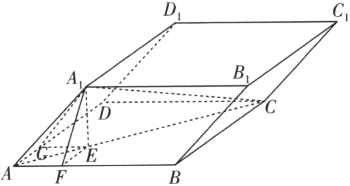
\includegraphics[width=42.0mm]{figs/image64.png}}\par\vspace{-1.0mm}\penalty10000

\begin{ansblock}[导-课时08-探4-例1]
% ans:导-课时08-探4-例1
\ansnote{例1}{\(\sqrt{2}\)}
\end{ansblock}

\liB{变式\textbf{1}}{中档(知识点一)}{}{如图，在长方形\(ABCD\)中，\(AB=2\)，\(BC=1\)，\(E\)为\(DC\)的中点，\(F\)为线段\(EC\)(端点除外)上一动点，现将\(\triangle AFD\)沿\(AF\)折起，使平面\(ABD\perp\)平面\(ABC\)，在平面\(ABD\)内过点\(D\)作\(DK\perp AB\)，\(K\)为垂足，设\(AK=t\)，则\(t\)的取值范围是\kongbai{}．}

\bindp \par\vspace{1.9mm}\penalty10000\noindent\makebox[\linewidth][c]{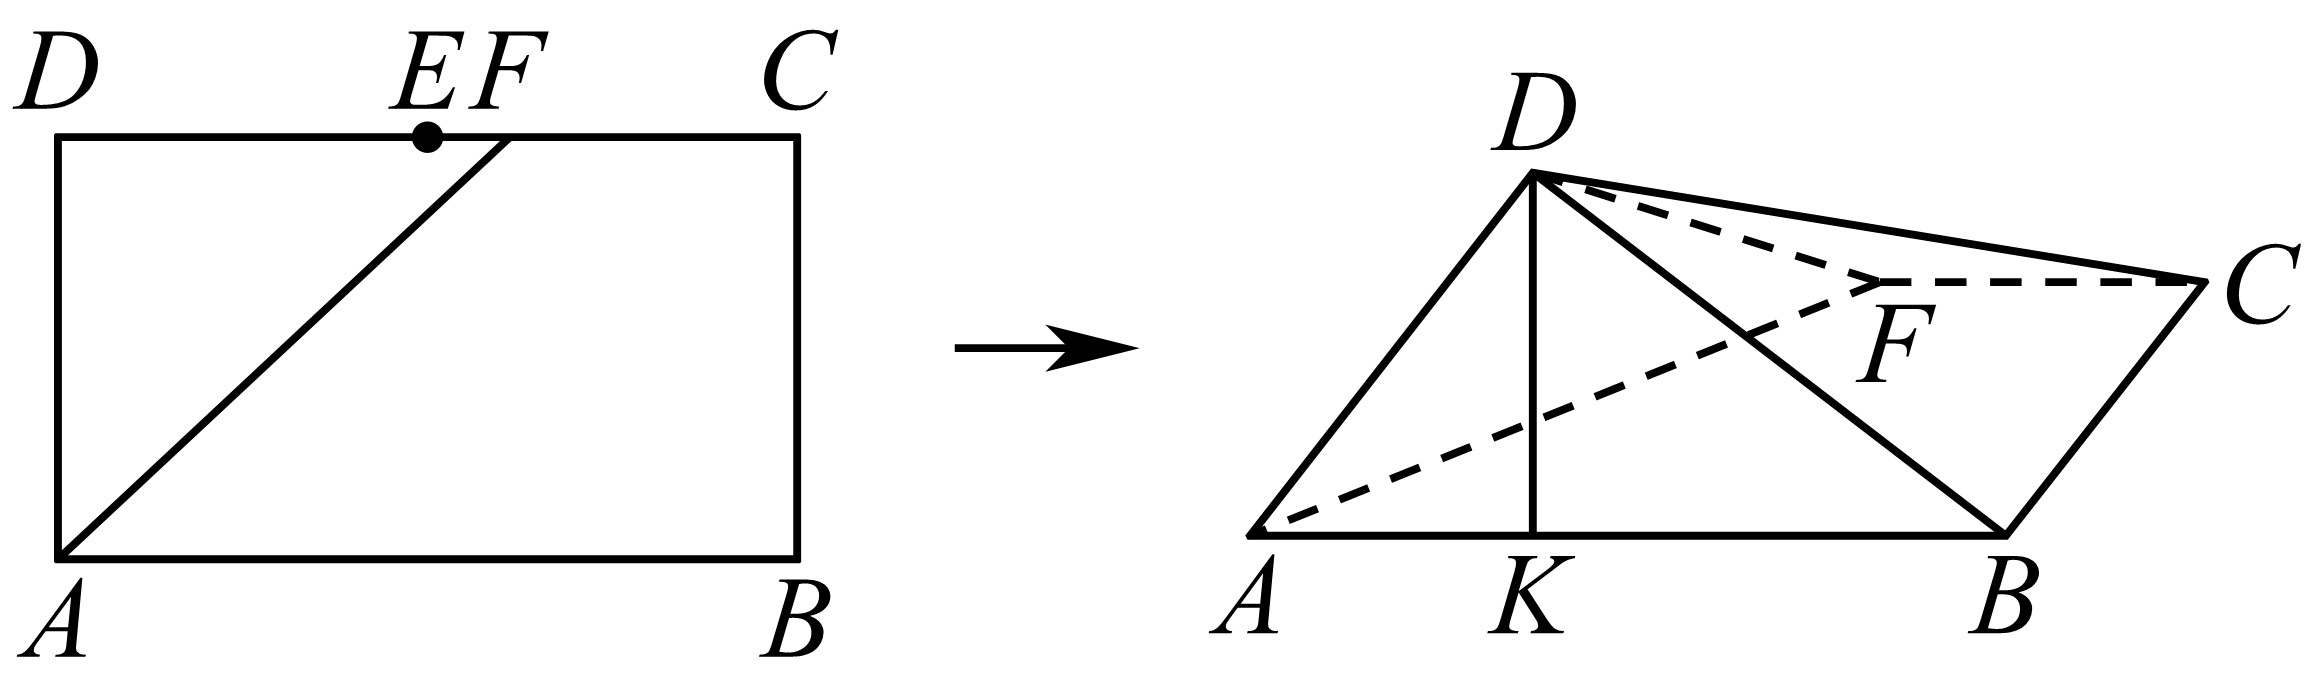
\includegraphics[width=60.0mm]{figs/image65.png}}\par\vspace{-1.0mm}\penalty10000

\begin{ansblock}[导-课时08-探4-变式1]
% ans:导-课时08-探4-变式1
\ansnote{变式1}{\(\left(\dfrac{1}{2},1\right)\)}
\end{ansblock}

\xiaojie{①识别：题干求线段长、棱长或线面角的取值范围与最值(含折叠中的连续变化)时，判归本题型.}

\bindpx {\kaishu ②操作：用三余弦定理定射影方向(或建系设顶点坐标)，把条件写成关于参数的等式；折叠问题锁定随动点连续变化的目标量.}

\bindpx {\kaishu ③收束：用正弦有界性、判别式、配方法或基本不等式求最值并注明取等条件；范围问题按端点能否取到写开闭区间.}

\tjdnr{五}{线面角的综合最值}{例\textbf{1}}{难(知识点二)}{如图，四棱锥\(P-ABCD\)的底面为正方形，\(PD\perp\)底面\(ABCD\)．设平面\(PAD\)与平面\(PBC\)的交线为\(l\)．(1)证明：\(l\perp\)平面\(PDC\)；(2)已知\(PD=AD=1\)，\(Q\)为\(l\)上的点，求\(PB\)与平面\(QCD\)所成角的正弦值的最大值．}

\bindp \par\vspace{1.9mm}\penalty10000\noindent\makebox[\linewidth][c]{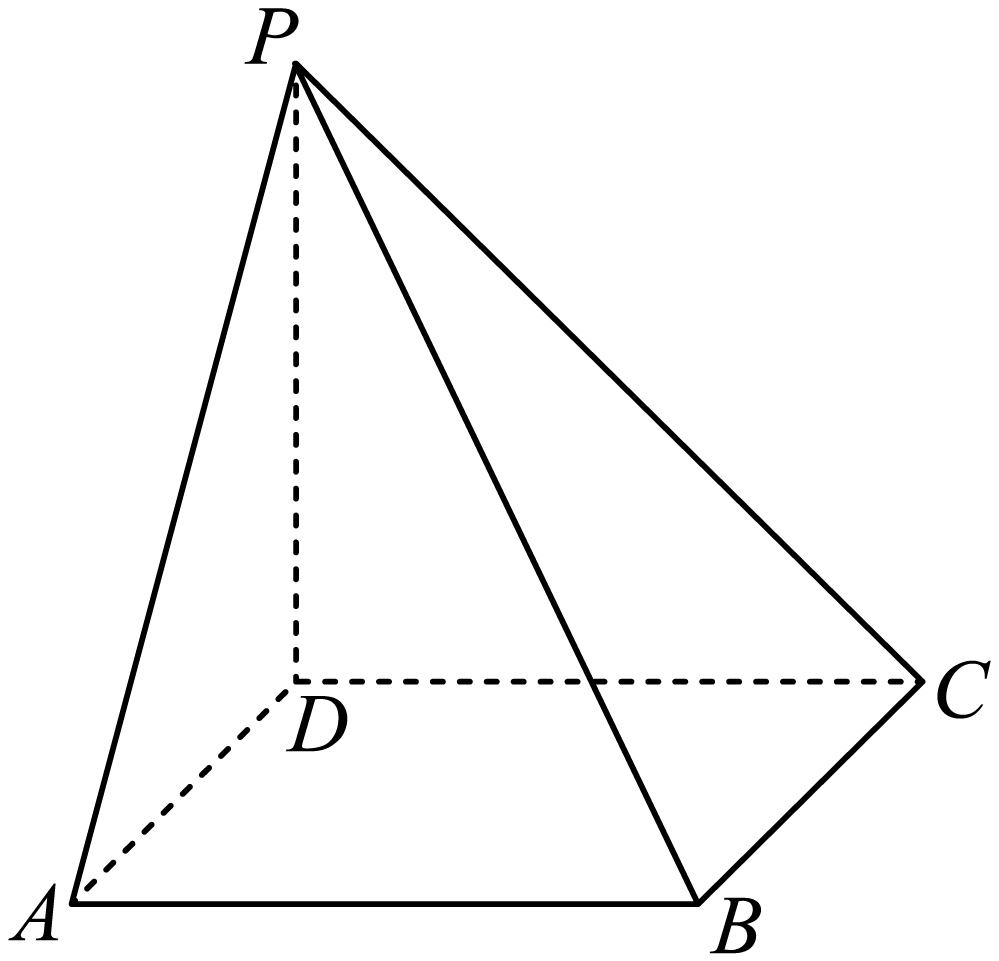
\includegraphics[width=34.0mm]{figs/image70.png}}\par\vspace{-1.0mm}\penalty10000

\liubai[12mm]{解答书写区}

\begin{ansblock}[导-课时08-探5-例1]
% ans:导-课时08-探5-例1
\ansnote{例1}{(1)证明见解析；(2)最大值 \(\dfrac{\sqrt{6}}{3}\)}
\end{ansblock}

\liB{变式\textbf{1}}{中档(知识点一)}{}{若直线\(l\)与平面\(\alpha\)所成的角为\(45^{\circ}\)，则\(l\)与平面\(\alpha\)内的直线所成角的取值范围是\kongbai{}．}

\begin{ansblock}[导-课时08-探5-变式1]
% ans:导-课时08-探5-变式1
\ansnote{变式1}{\([45^{\circ},90^{\circ}]\)}
\end{ansblock}

\xiaojie{①识别：题干含动点(动平面)、要求线面角的正弦(余弦)的最值或范围时，判归本题型.}

\bindpx {\kaishu ②操作：建系并用参数表示动点，求出相应平面的法向量，把线面角的正弦写成参数的函数.}

\bindpx {\kaishu ③收束：用基本不等式或代数变形求最值并注明取等条件；求范围时结合最小角定理定下界.}

% ---------- 课堂评价（恒 5 题＝3 单选＋2 填空；3 简单＋2 中档≤例题；提示词形制；全命制——逐题亲算登批4值台账） ----------
\begin{ketang}{本组共5题，1—3为单选，4—5为填空．}

\jiancestem{{\fontsize{11.4pt}{14pt}\selectfont\heihao {\numboldjian 1}．}\hspace{4.1mm}\tieside{简单(知识点一)}\hspace{2.2mm}直线\(l\)与平面\(\alpha\)所成的角为\(\theta\)，则\(\theta\)的取值范围是(\kongwei)}

\bindopt {\fontsize{10.5pt}{21pt}\selectfont \makebox[\dimexpr0.5\linewidth-1em\relax][l]{A．\([0^{\circ},90^{\circ})\)；}\makebox[\dimexpr0.5\linewidth-1em\relax][l]{B．\((0^{\circ},90^{\circ}]\)；}\par}

\bindopt {\fontsize{10.5pt}{21pt}\selectfont \makebox[\dimexpr0.5\linewidth-1em\relax][l]{C．\([0^{\circ},90^{\circ}]\)；}\makebox[\dimexpr0.5\linewidth-1em\relax][l]{D．\([0^{\circ},180^{\circ}]\)}\par}

\begin{ansblock}[导-课时08-评1]
% ans:导-课时08-评1
\ansitem{1}{C（\([0^{\circ},90^{\circ}]\)）}
\end{ansblock}

\jiancestem{{\fontsize{11.4pt}{14pt}\selectfont\heihao {\numboldjian 2}．}\hspace{4.1mm}\tieside{简单(知识点二)}\hspace{2.2mm}直线\(l\)的方向向量为\(\overrightarrow{u}=(1,1,\sqrt{2})\)，平面\(\alpha\)的一个法向量为\(\overrightarrow{n}=(0,0,1)\)，则\(l\)与\(\alpha\)所成角的正弦值为(\kongwei)}

\bindopt {\fontsize{10.5pt}{21pt}\selectfont \makebox[\dimexpr0.5\linewidth-1em\relax][l]{A．\(\frac{\sqrt{2}}{2}\)；}\makebox[\dimexpr0.5\linewidth-1em\relax][l]{B．\(\frac{1}{2}\)；}\par}

\bindopt {\fontsize{10.5pt}{21pt}\selectfont \makebox[\dimexpr0.5\linewidth-1em\relax][l]{C．\(\frac{\sqrt{3}}{2}\)；}\makebox[\dimexpr0.5\linewidth-1em\relax][l]{D．\(\frac{\sqrt{3}}{3}\)}\par}

\begin{ansblock}[导-课时08-评2]
% ans:导-课时08-评2
\ansitem{2}{A}
\end{ansblock}

\jiancestem{{\fontsize{11.4pt}{14pt}\selectfont\heihao {\numboldjian 3}．}\hspace{4.1mm}\tieside{中档(知识点三)}\hspace{2.2mm}正方体\(ABCD-A_{1}B_{1}C_{1}D_{1}\)中，直线\(BC_{1}\)与平面\(ABCD\)的对角线\(AC\)所成的角为(\kongwei)}

\bindopt {\fontsize{10.5pt}{21pt}\selectfont \makebox[\dimexpr0.25\linewidth-0.5em\relax][l]{A．\(30^{\circ}\)；}\makebox[\dimexpr0.25\linewidth-0.5em\relax][l]{B．\(45^{\circ}\)；}\makebox[\dimexpr0.25\linewidth-0.5em\relax][l]{C．\(60^{\circ}\)；}\makebox[\dimexpr0.25\linewidth-0.5em\relax][l]{D．\(90^{\circ}\)}\par}

\begin{ansblock}[导-课时08-评3]
% ans:导-课时08-评3
\ansitem{3}{C（\(60^{\circ}\)）}
\end{ansblock}

\jiancestem{{\fontsize{11.4pt}{14pt}\selectfont\heihao {\numboldjian 4}．}\hspace{4.1mm}\tieside{简单(知识点一)}\hspace{2.2mm}直线\(l\)与平面\(\alpha\)所成的角为\(30^{\circ}\)，则平面\(\alpha\)内与\(l\)所成的角为\(90^{\circ}\)的直线有\kongbai{}条．{\zhushi{(提示：考虑平面\(\alpha\)内与\(l\)在\(\alpha\)内的射影垂直的直线与\(l\)的位置关系)}}}

\begin{ansblock}[导-课时08-评4]
% ans:导-课时08-评4
\ansitem{4}{无数}
\end{ansblock}

\jiancestem{{\fontsize{11.4pt}{14pt}\selectfont\heihao {\numboldjian 5}．}\hspace{4.1mm}\tieside{中档(知识点二)}\hspace{2.2mm}已知直线\(l\)的方向向量\(\overrightarrow{u}=(1,2,2)\)，平面\(\alpha\)的法向量\(\overrightarrow{n}=(2,-1,2)\)，则直线\(l\)与平面\(\alpha\)所成角的正弦值为\kongbai{}．{\zhushi{(提示：\(\sin\theta=|\cos\langle\overrightarrow{u},\overrightarrow{n}\rangle|=\frac{|\overrightarrow{u}\cdot\overrightarrow{n}|}{|\overrightarrow{u}||\overrightarrow{n}|}\))}}}

\begin{ansblock}[导-课时08-评5]
% ans:导-课时08-评5
\ansitem{5}{\(\dfrac{4}{9}\)}
\end{ansblock}

\end{ketang}

\end{multicols}

\tailfill
\end{document}
